\section{Method}\label{sec:method}
As of now, the project has made progress towards user-friendliness and accuracy, and all that is needed
is a smartphone with the application installed and a paper sheet.
The pipeline is still divided into a preliminary phase and a real-time phase,
but now all the work is done by a single device instead of three different devices.

Launching the application immediately gives visual feedback from the camera on the smartphone screen:
the user directly sees what they are framing with the camera, making the preliminary phase much faster and easier,
also thanks to a visual guide in transparency on the image, which is used to aim at the keyboard.

Once the keyboard is centered in the visual guide, the user can press a button on the application interface
to start the process of detecting the keyboard.
The detection process takes less than a second, and once it is finished, the screen will display in transparency the
keys detected by the application, so that the user can assess whether the process was successful and,
if they are not satisfied, repeat it as many times as necessary.

Both the visual guide and the keys in transparency can be hidden either before or after the preliminary step.
When the user is satisfied with the result of the preliminary stage, they can immediately start playing on the
semi-virtual keyboard, without any other interaction with the application.

The entire process is shown in~\autoref{fig:keyrtual-smartphone-method}
and the implementation details are explained in the following paragraphs.

\begin{figure}[ht]
	\centering
	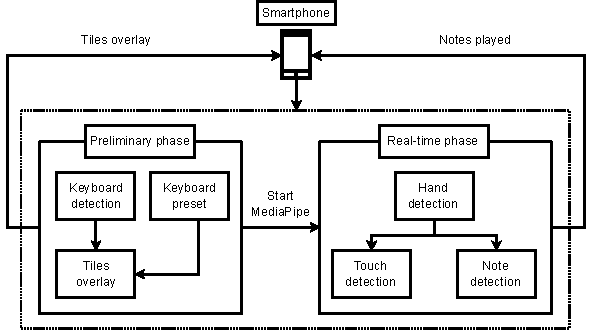
\includegraphics[width=0.8\textwidth]{images/application/architecture}
	\caption{Architecture of the current version}
	\label{fig:keyrtual-smartphone-method}
\end{figure}

\subsection{Constraints}\label{subsec:constraints}

\paragraph{General constraints}
The sheet should be a common white A4 sheet and the keyboard should be drawn in black or blue for better contrast.
There are no constraints on the contrast between the paper sheet and table due to the new background subtraction method.

The phone should be placed at a sufficient distance to frame the paper and hands in their entirety (experimentally
we have found that about 40 cm is fine) in a way such that the user, relative to the camera, appears to be on the top side
of the image and the paper on the bottom side of the image.

\paragraph{Hardware prerequisites}
No special prerequisites are required to run the application.
Thanks to the possibility of increasing and decreasing the FPS with which to run MediaPipe,
which is the most computationally demanding component,
it is possible to sacrifice some response speed to ensure that the application works on low-end phones.

\subsection{Preliminary phase}\label{subsec:preliminary-phase}
The preliminary phase still consists of background subtraction and keyboard detection, but the process to follow is much
faster, intuitive and automated.

All the single steps of this phase are shown in~\autoref{fig:preprocessing}.

\paragraph{Image acquisition}
As soon as the application is opened, the user can immediately go to the preliminary step of keyboard detection.
Due to the high mobility of the smartphone and the immediate visual feedback from the screen,
no real background subtraction process is required during this phase: a perimeter is drawn on the smartphone screen
around the area within which the application expects the user to frame the drawn keyboard.

When the user frames the keyboard in the perimeter and presses the button to start the detection process,
the application takes an image with a resolution of $1280 \times 720$, a reasonable resolution for all modern smartphones,
and cuts off from the image all the area outside the perimeter, keeping only the area where the keyboard is located.
This makes the background subtraction process much more effective and accurate,
and also much faster since no particular algorithm is used.

Since smartphone webcams, used via Unity, have an image correction and automatic focus function,
we had to take countermeasures to prevent the webcam from automatically
moving the focus outside our perimeter, making the detection phase inaccurate.
To do this, we forced the webcam's focus on the centre of the perimeter via Unity's API\@.

The perimeter and the result for this phase are shown in \autoref{fig:perimeter} and \autoref{fig:mat}.

\paragraph{Preprocessing}
Before performing the actual keyboard detection, we go through a second but very important preprocessing step:
filters are applied to the cropped keyboard image to highlight the 
keys drawn in black against the white background of the paper sheet.

The image is converted to grayscale and Canny edge detector algorithm is applied to highlight the black lines.
Two iterations of closing morphological operator are applied to the image, to enhance the visibility of the edges found by Canny.
We are not quite interested in cleaning those small white pixel spots that appear scattered over the image
because they will be removed during the next step.

The single steps of this phase can be seen in \autoref{fig:canny} and \autoref{fig:canny-closed}.

\paragraph{Tiles detection}
At this point, we proceed to the actual keyboard detection.
After extensive experimentation, we concluded that the old method using probabilistic Hough Transform to detect lines
was too inaccurate and inconsistent, and moreover wouldn't allow us to detect non-straight lines,
which is a fundamental prerequisite in this case since we would like to detect hand-drawn keyboards.
Therefore, we opted for a much simpler and more robust method: contour detection~\cite{contour-detection}.

The contour detection procedure is applied to edges obtained from the previous step.
The contours thus obtained, however, are filtered in several ways, eliminating:
\begin{itemize}
	\item contours with width greater than height (non-vertical)
	\item contours with area smaller than 300 pixels
	\item contours with area greater than 5\% of the image
\end{itemize}
The contours left represent the keys drawn on the paper and are shown in \autoref{fig:contours}.

\paragraph{Tiles overlay}
With the previously obtained contours, the overlay with the keys drawn in transparency is created and shown to the user.
To make the overlay look like a real keyboard, the keys are colored white or black according to their length:
longer keys are white and shorter keys are black.

The result can be seen in \autoref{fig:tiles-overlay}

\paragraph{Notes detection}\label{par:notes-detection}
The contours are sorted using the horizontal center as the sorting criteria.
An image is then created with the same size as the original, initially all black,
which is colored only inside the areas of the contours found.
The areas are colored with a gray scale starting at 1 and going up by 1 for each key.

The color for each key represents an index, starting from 1 up to the number of keys found,
which is used to determine the note number to be played according to the MIDI protocol.
The details of this method are explained in \autoref{subsubsec:notes-detection}~\nameref{subsubsec:notes-detection}.

The final result is shown in \autoref{fig:notes}.

\begin{figure}[ht]
	\centering
	\begin{subfigure}{0.49\textwidth}
		\centering
		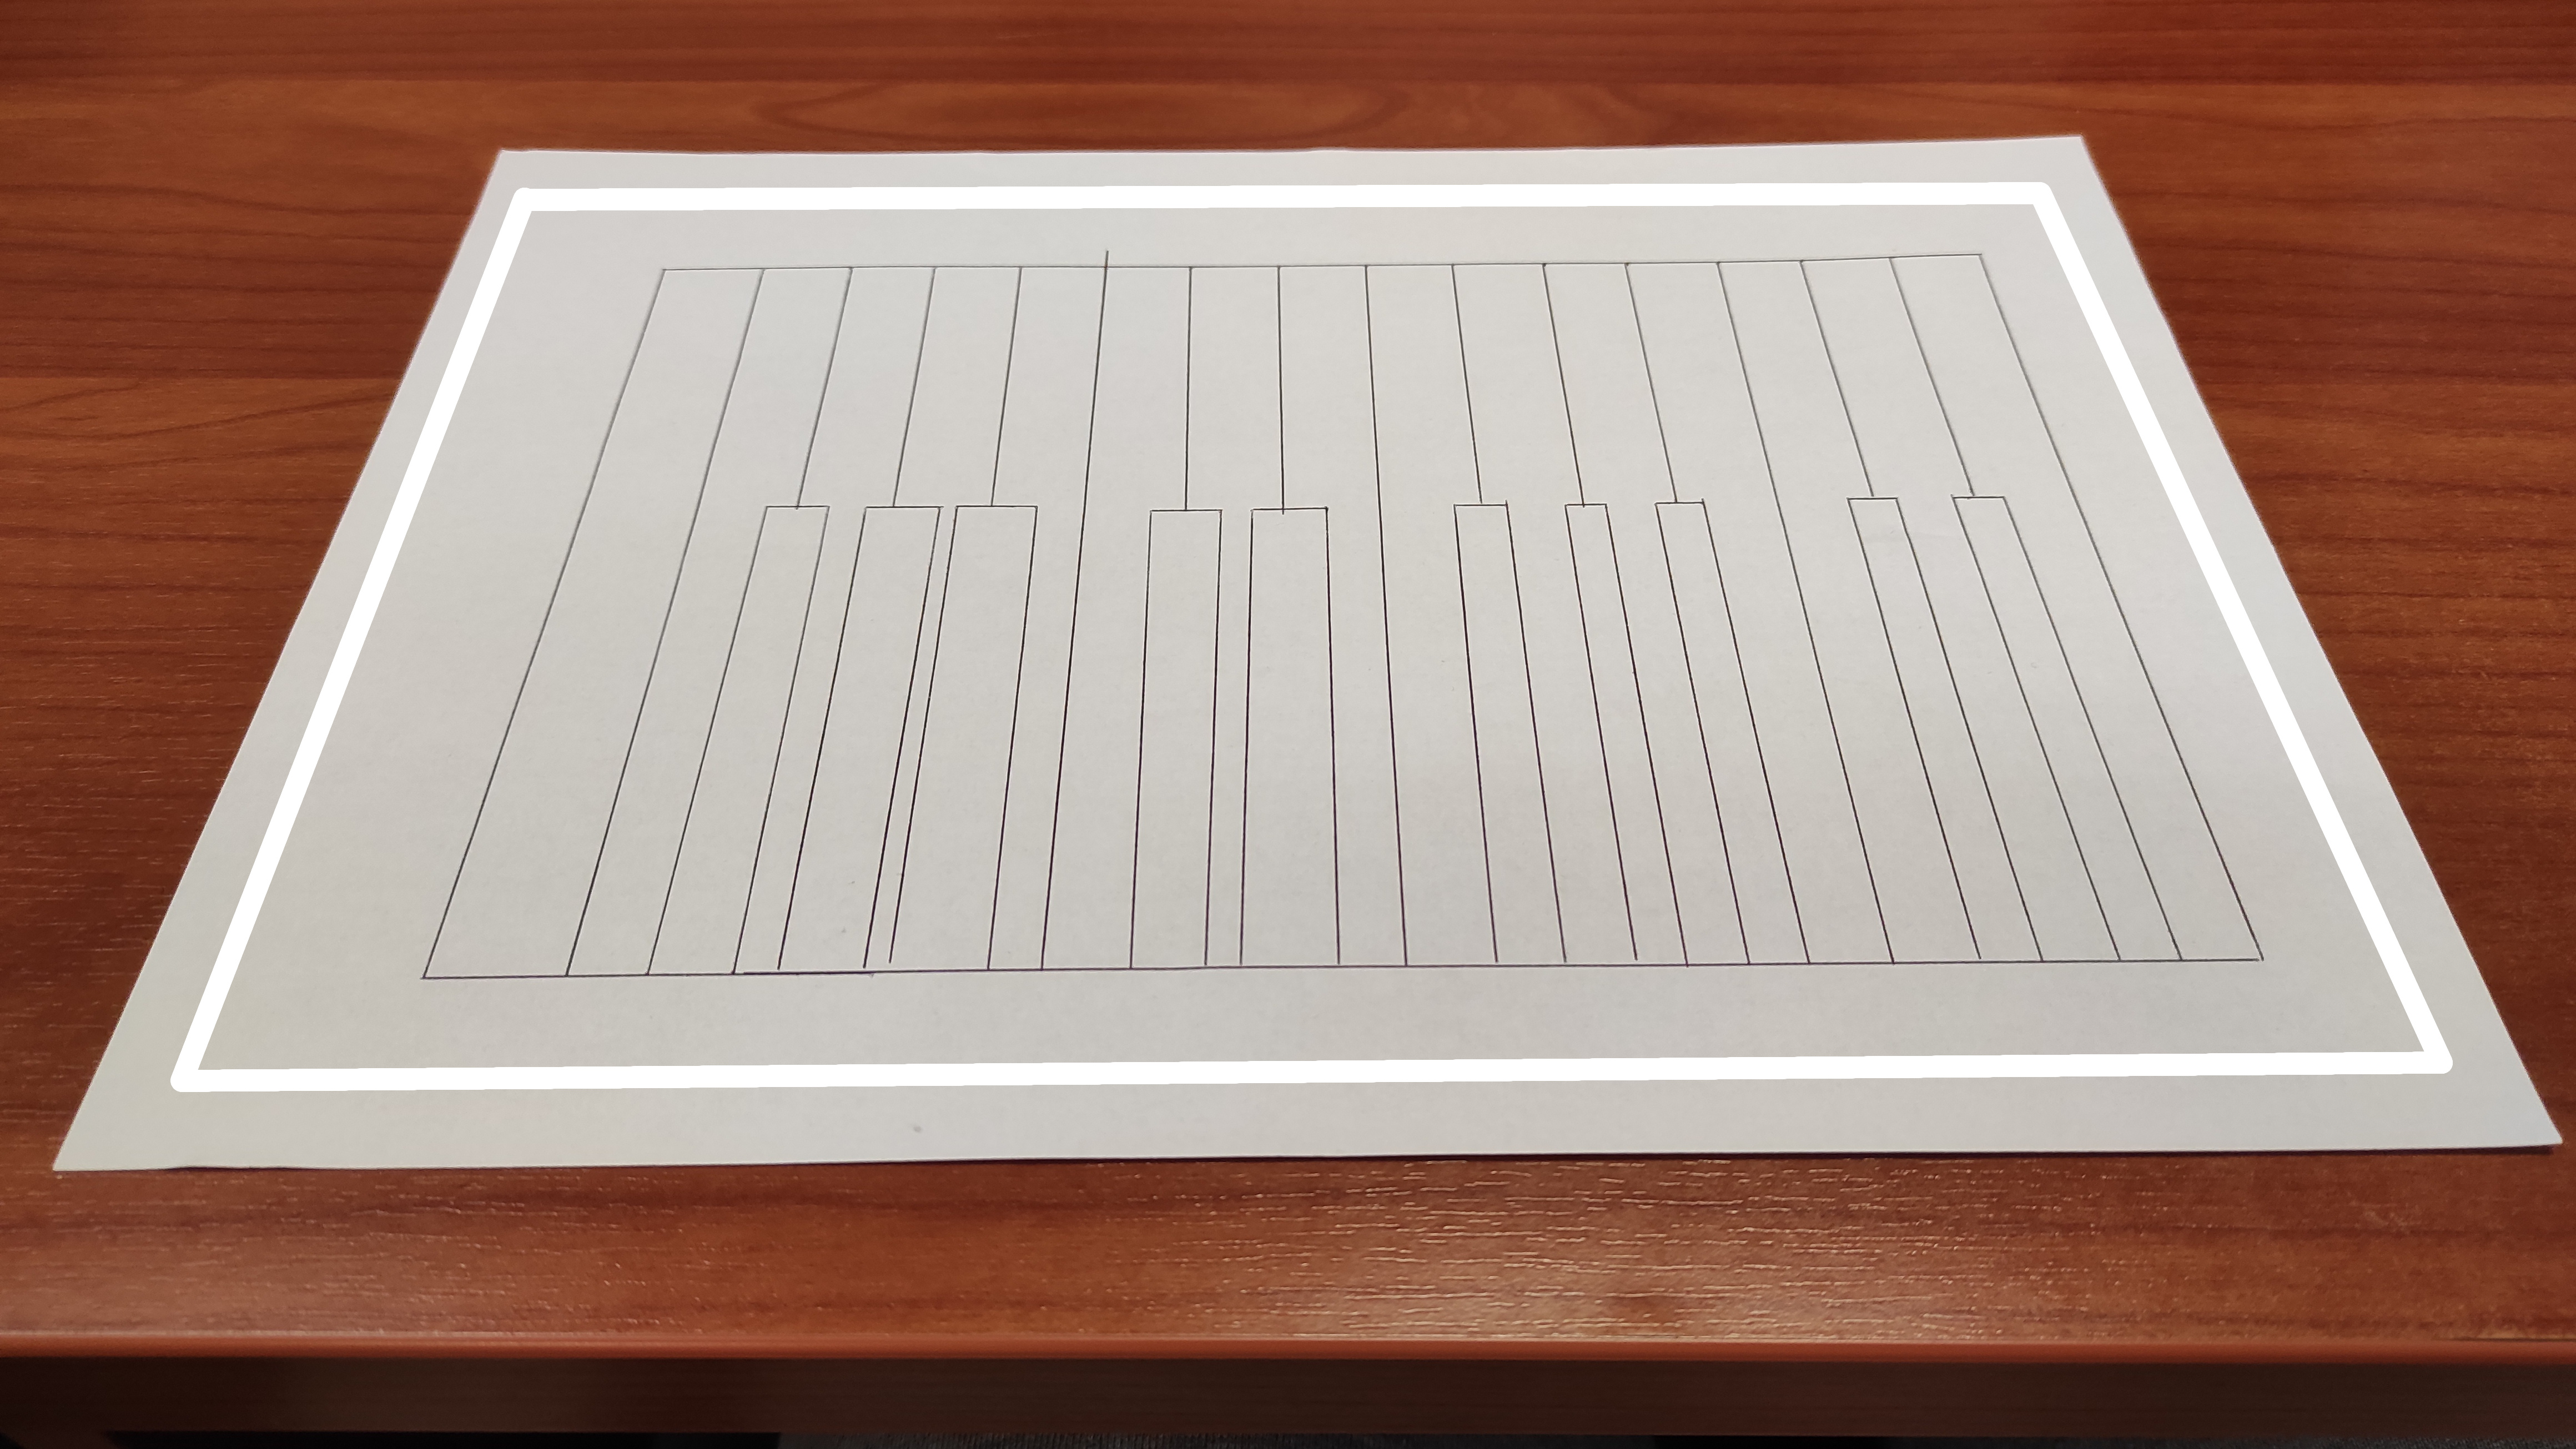
\includegraphics[width=\textwidth]{images/application/45deg/camera-with-frame}
		\caption{}
		\label{fig:perimeter}
	\end{subfigure}
	\hfill
	\begin{subfigure}{0.49\textwidth}
		\centering
		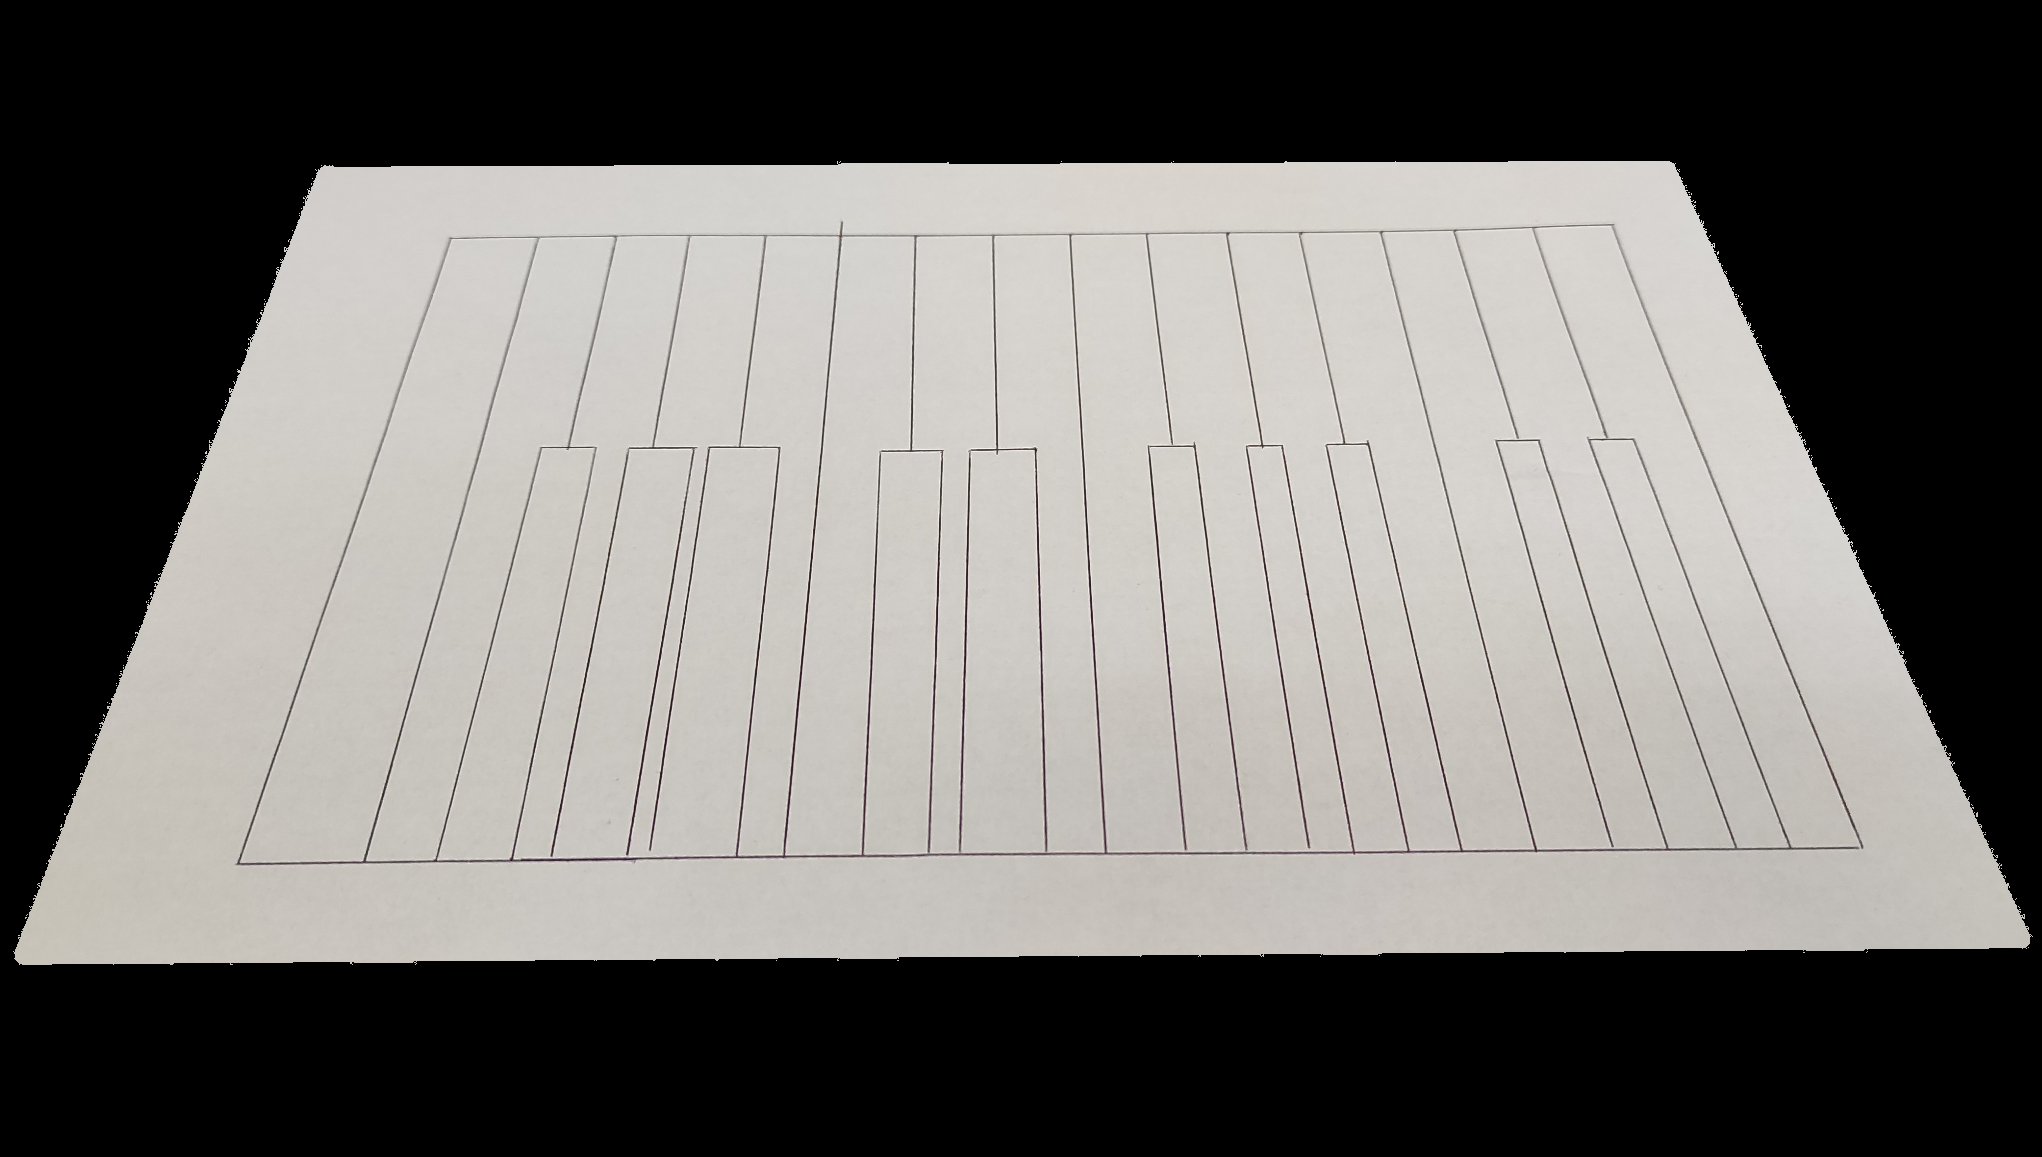
\includegraphics[width=\textwidth]{images/application/45deg/masked}
		\caption{}
		\label{fig:mat}
	\end{subfigure}
	\hfill
	\begin{subfigure}{0.49\textwidth}
		\centering
		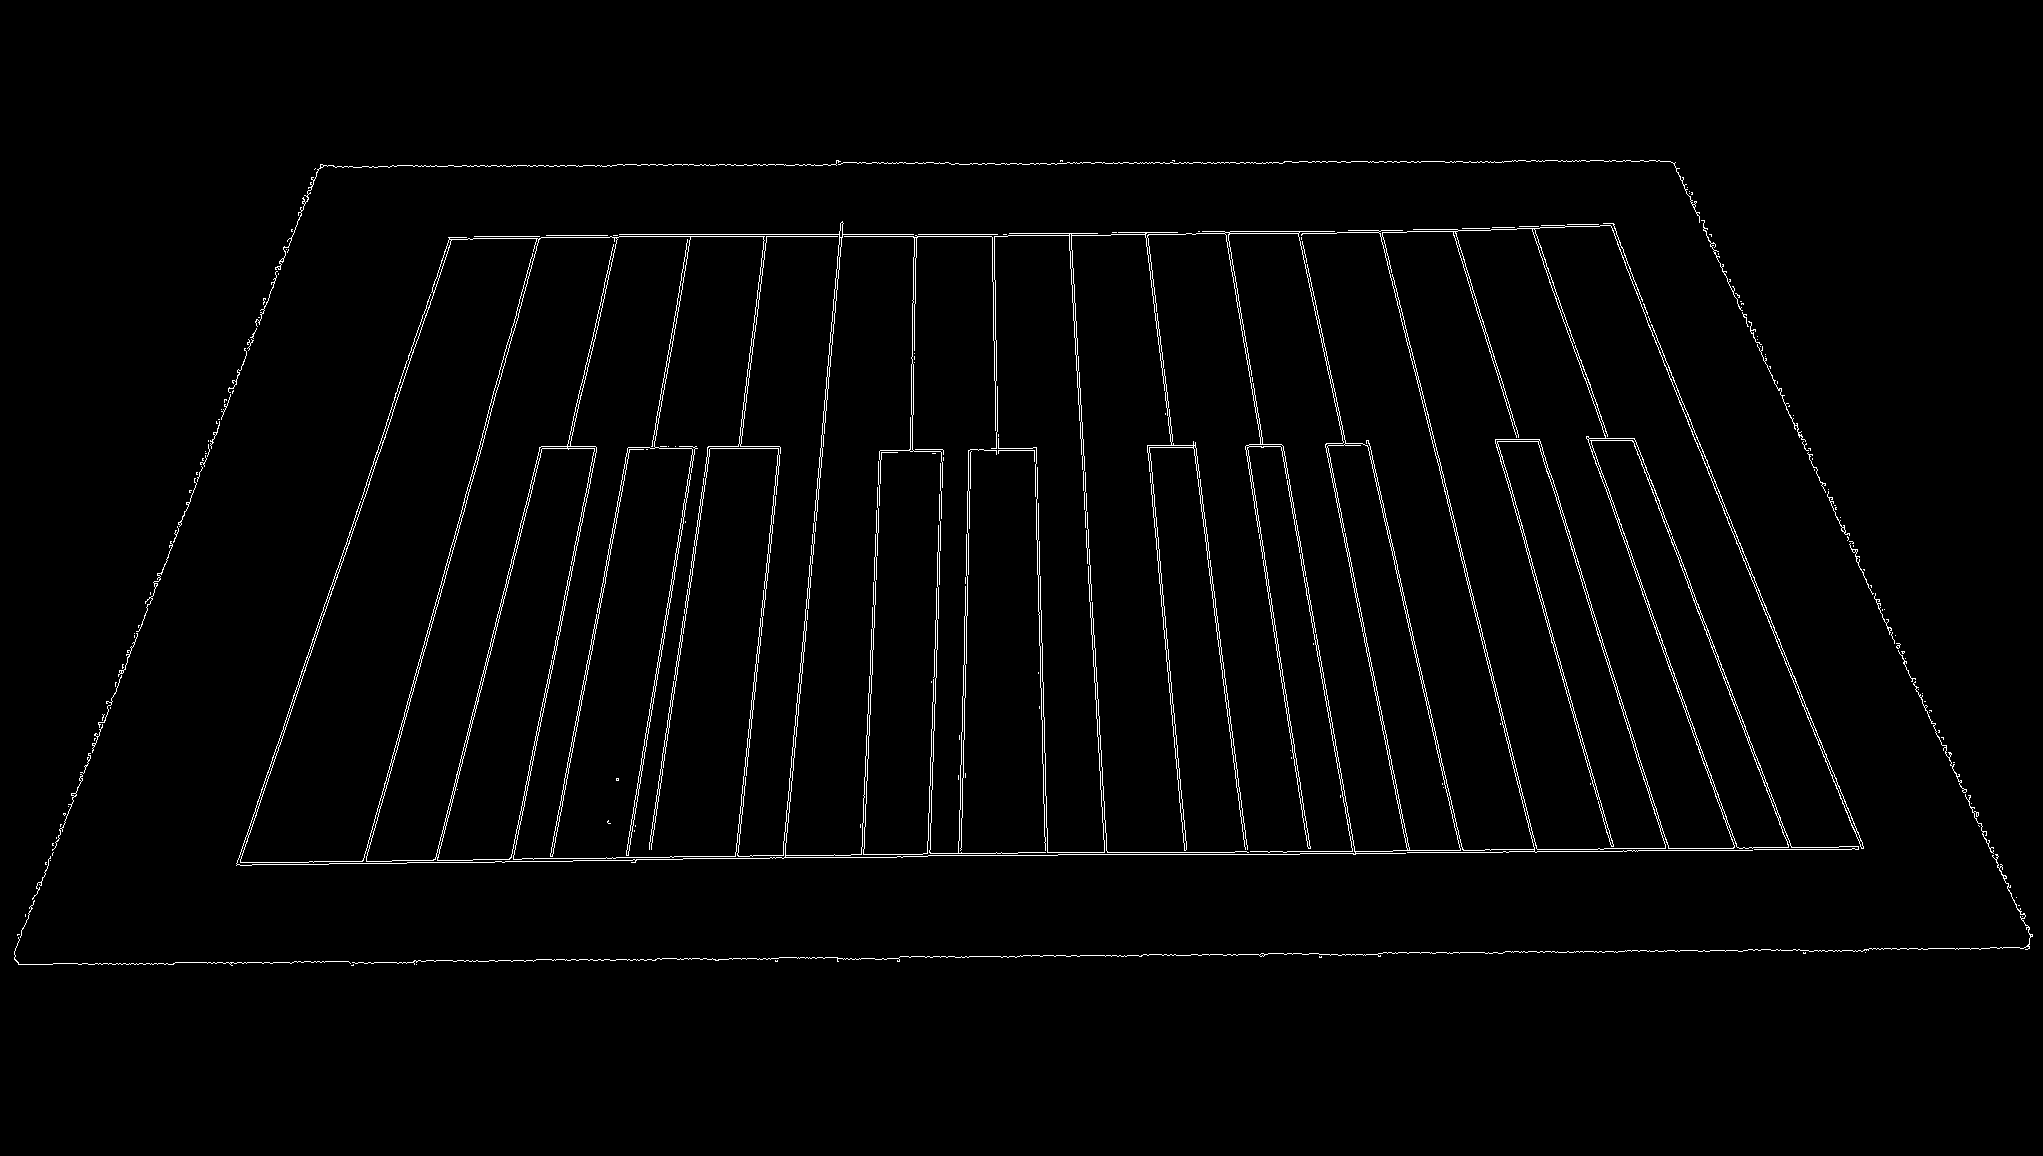
\includegraphics[width=\textwidth]{images/application/45deg/canny}
		\caption{}
		\label{fig:canny}
	\end{subfigure}
	\hfill
	\begin{subfigure}{0.49\textwidth}
		\centering
		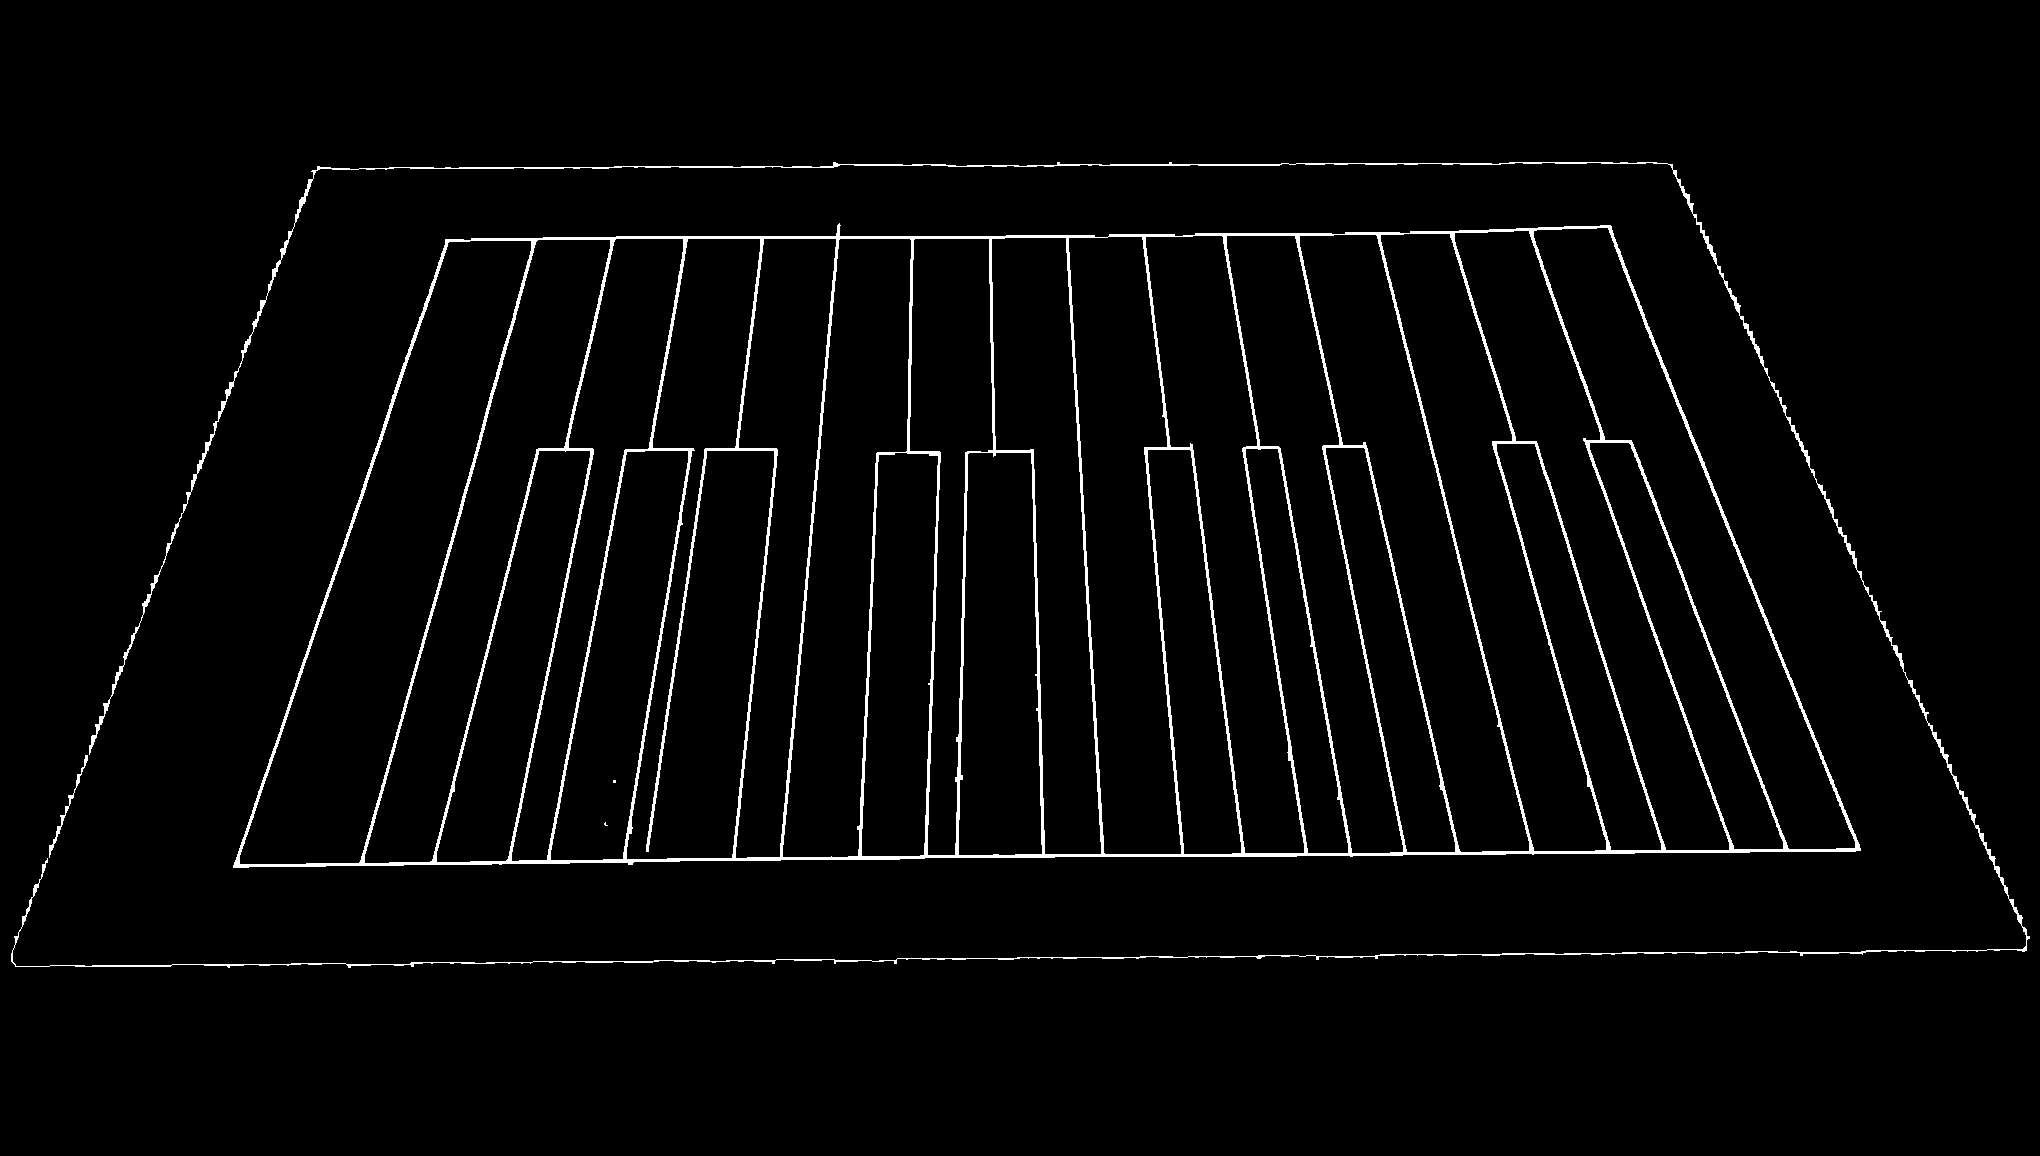
\includegraphics[width=\textwidth]{images/application/45deg/canny-closed}
		\caption{}
		\label{fig:canny-closed}
	\end{subfigure}
	\hfill
	\begin{subfigure}{0.49\textwidth}
		\centering
		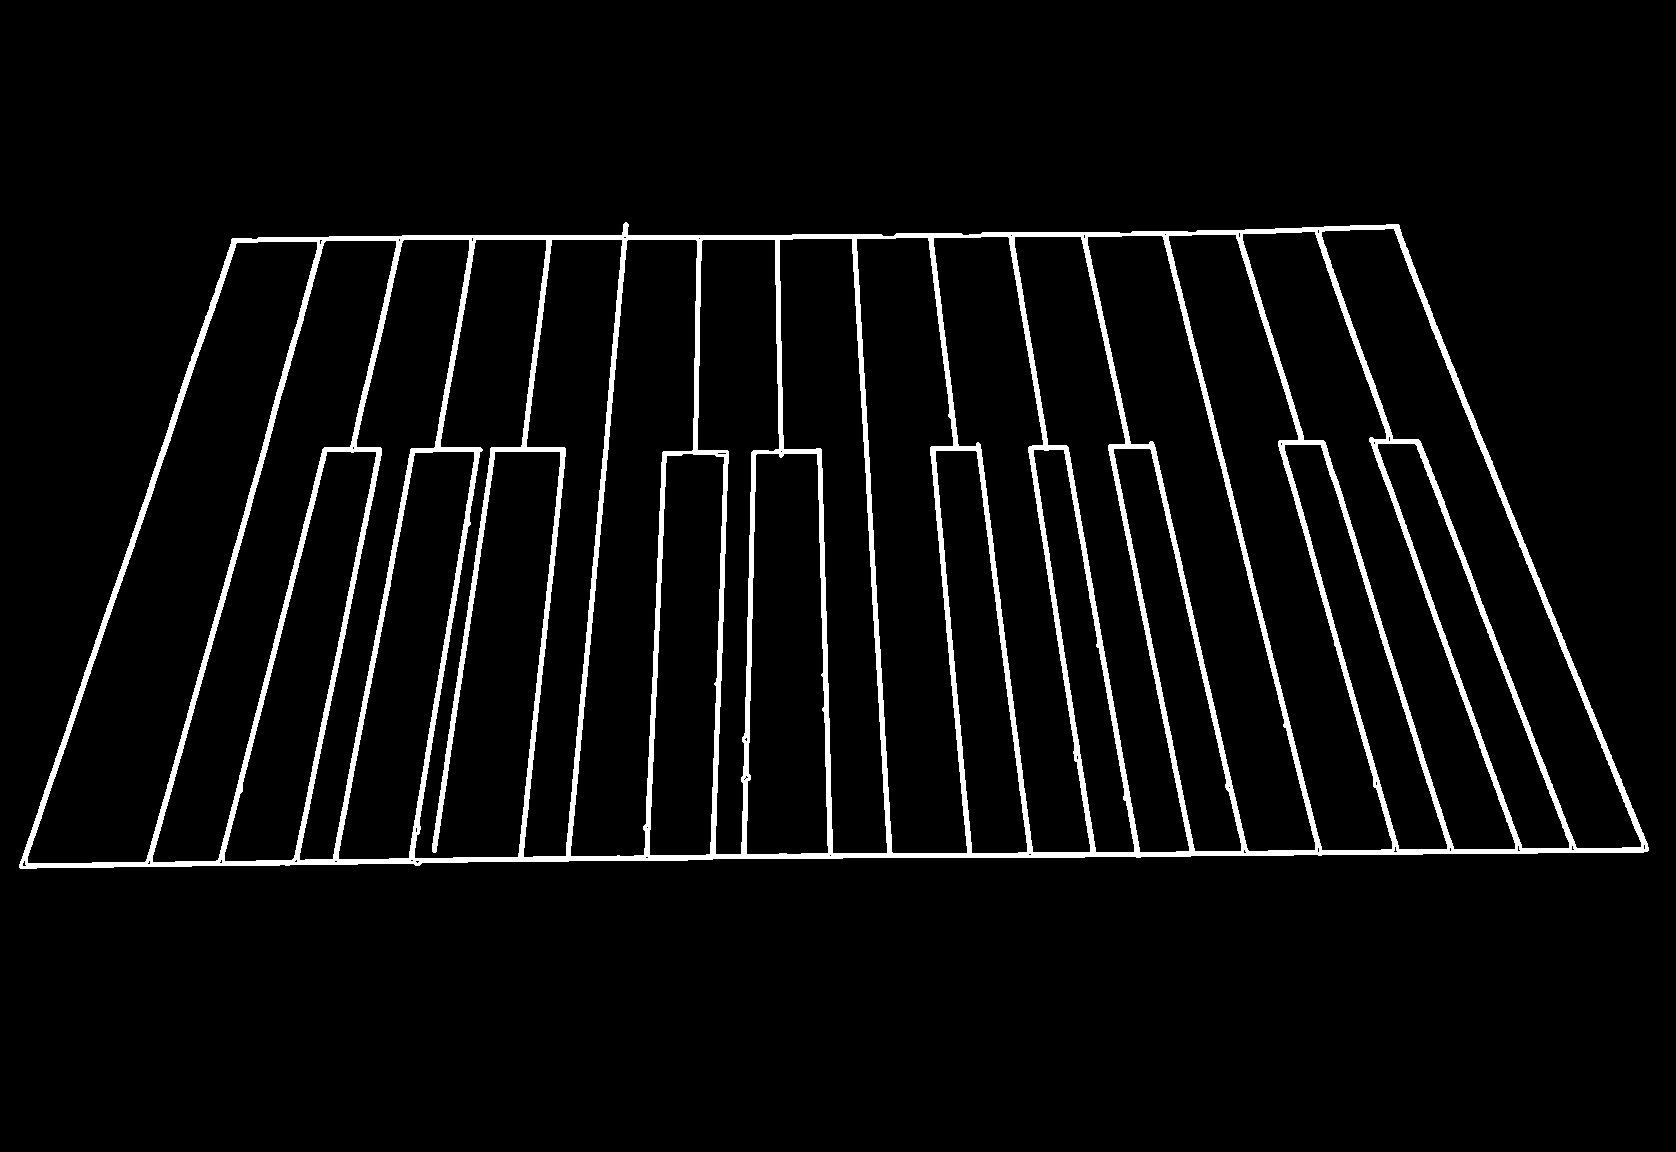
\includegraphics[width=\textwidth]{images/application/45deg/contours}
		\caption{}
		\label{fig:contours}
	\end{subfigure}
	\hfill
	\begin{subfigure}{0.49\textwidth}
		\centering
		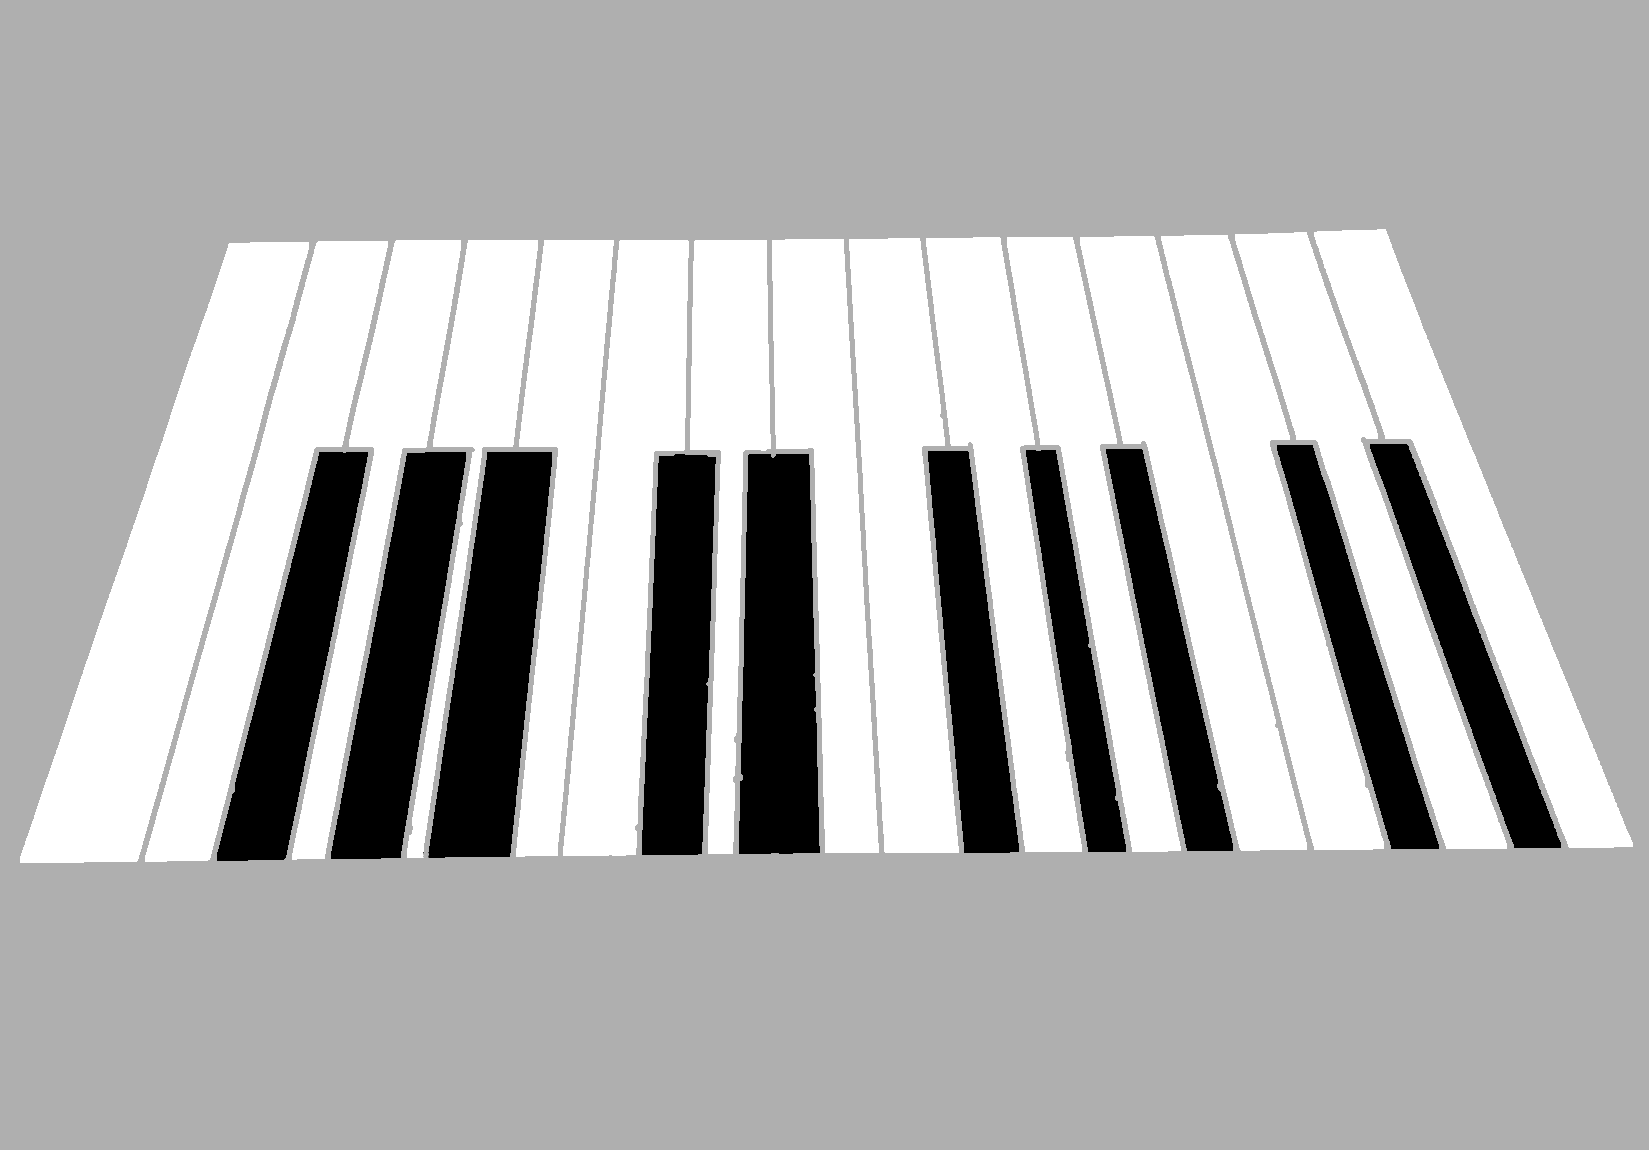
\includegraphics[width=\textwidth]{images/application/45deg/tiles-overlay}
		\caption{}
		\label{fig:tiles-overlay}
	\end{subfigure}
	\hfill
	\begin{subfigure}{0.49\textwidth}
		\centering
		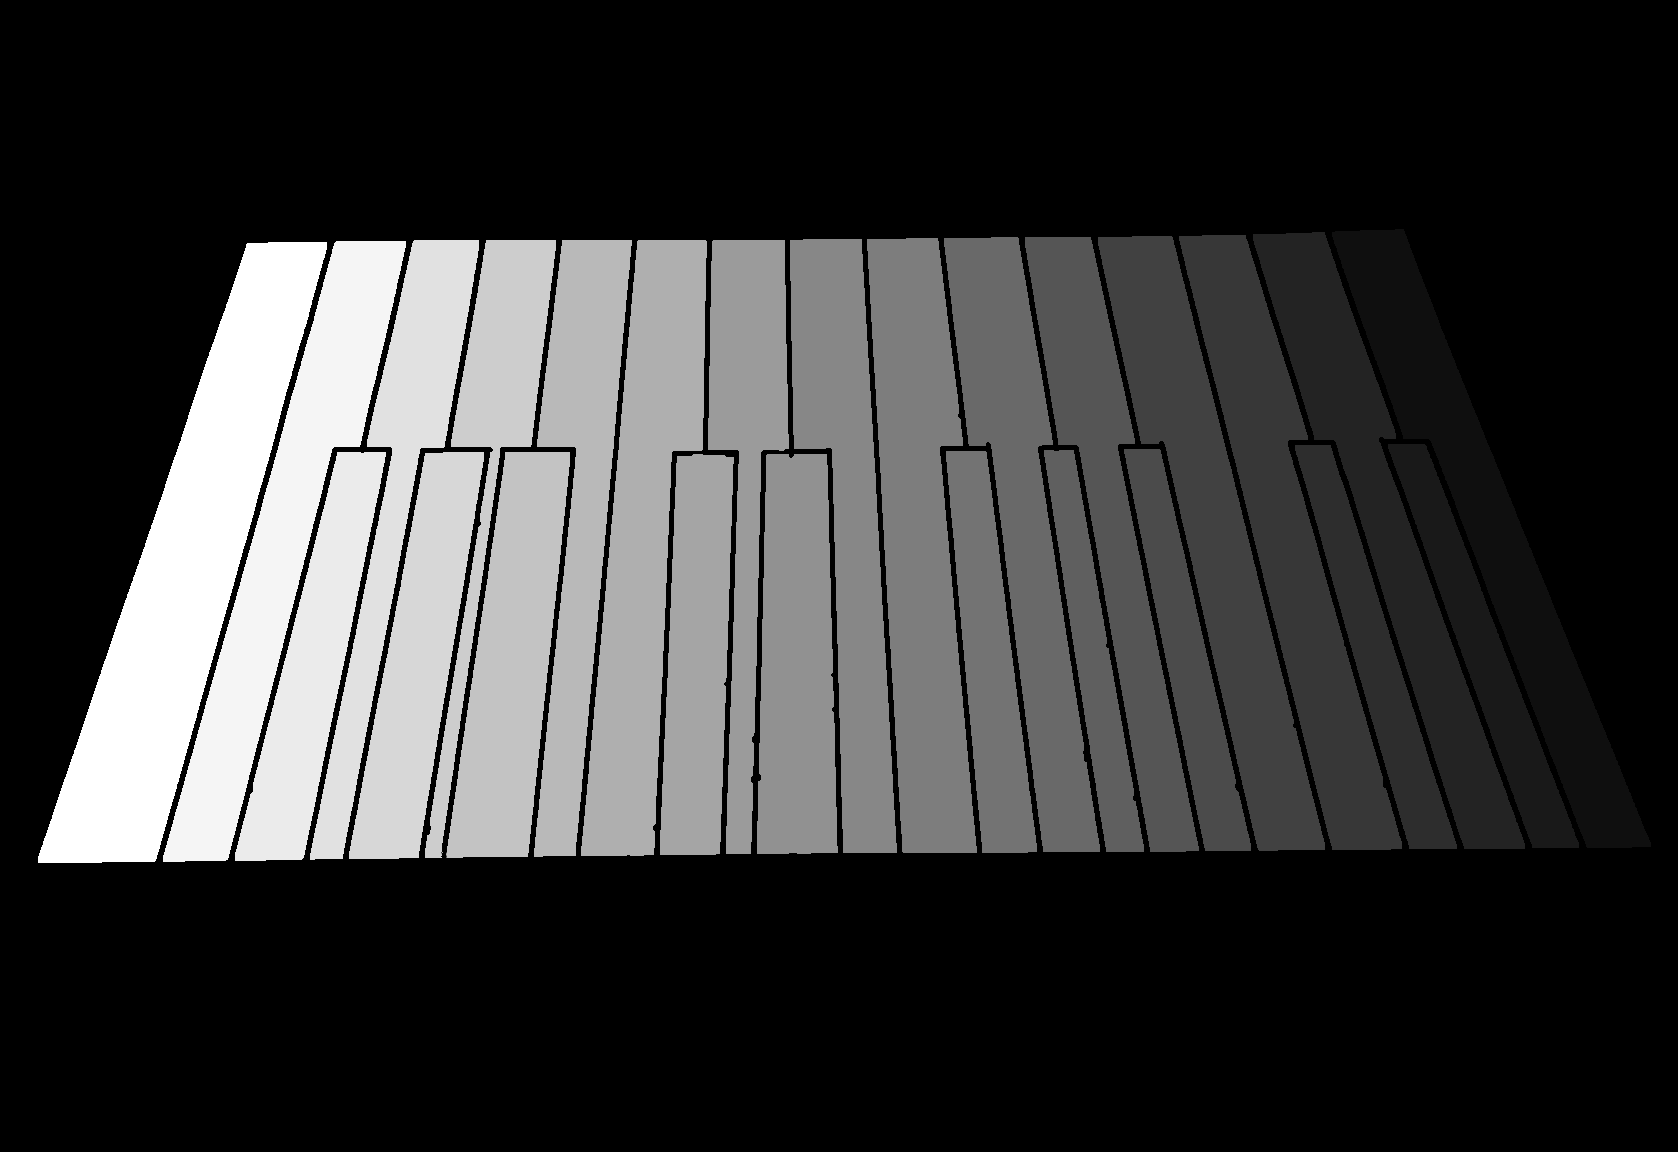
\includegraphics[width=\textwidth]{images/application/45deg/notes-overlay}
		\caption{}
		\label{fig:notes}
	\end{subfigure}
	\caption{
		Keyboard detection pipeline.
		(a) Perimeter;
		(b) Keyboard after background subtraction;
		(c) Canny edge;
		(d) Canny edge after morphological closure;
		(e) Contour detection (after filter);
		(f) Tiles overlay (not in transparency for visibility);
		(g) Notes indexes (brightness enhanced for visibility).
	}
	\label{fig:preprocessing}
\end{figure}

\subsubsection{Keyboard presets}
In this mode, instead of using a photo taken by the user to search for the keyboard and show the keys thus detected,
the shape and position of the keys that the application expects to use is shown directly.

The user can download and print out on an A4 sheet the model of the keyboard that the
application shows on the screen and must position it at the guides shown on the interface.
In this way, the user's physical keyboard will perfectly match the one presented by the application,
ensuring optimal performance and realism.

The PDF files for printing the keyboard presets will be available for download on the project's website.
The different keyboard models made available by default by the application are shown in \autoref{fig:presets}.

\begin{figure}[ht]
	\centering
	\begin{subfigure}{0.49\textwidth}
		\centering
		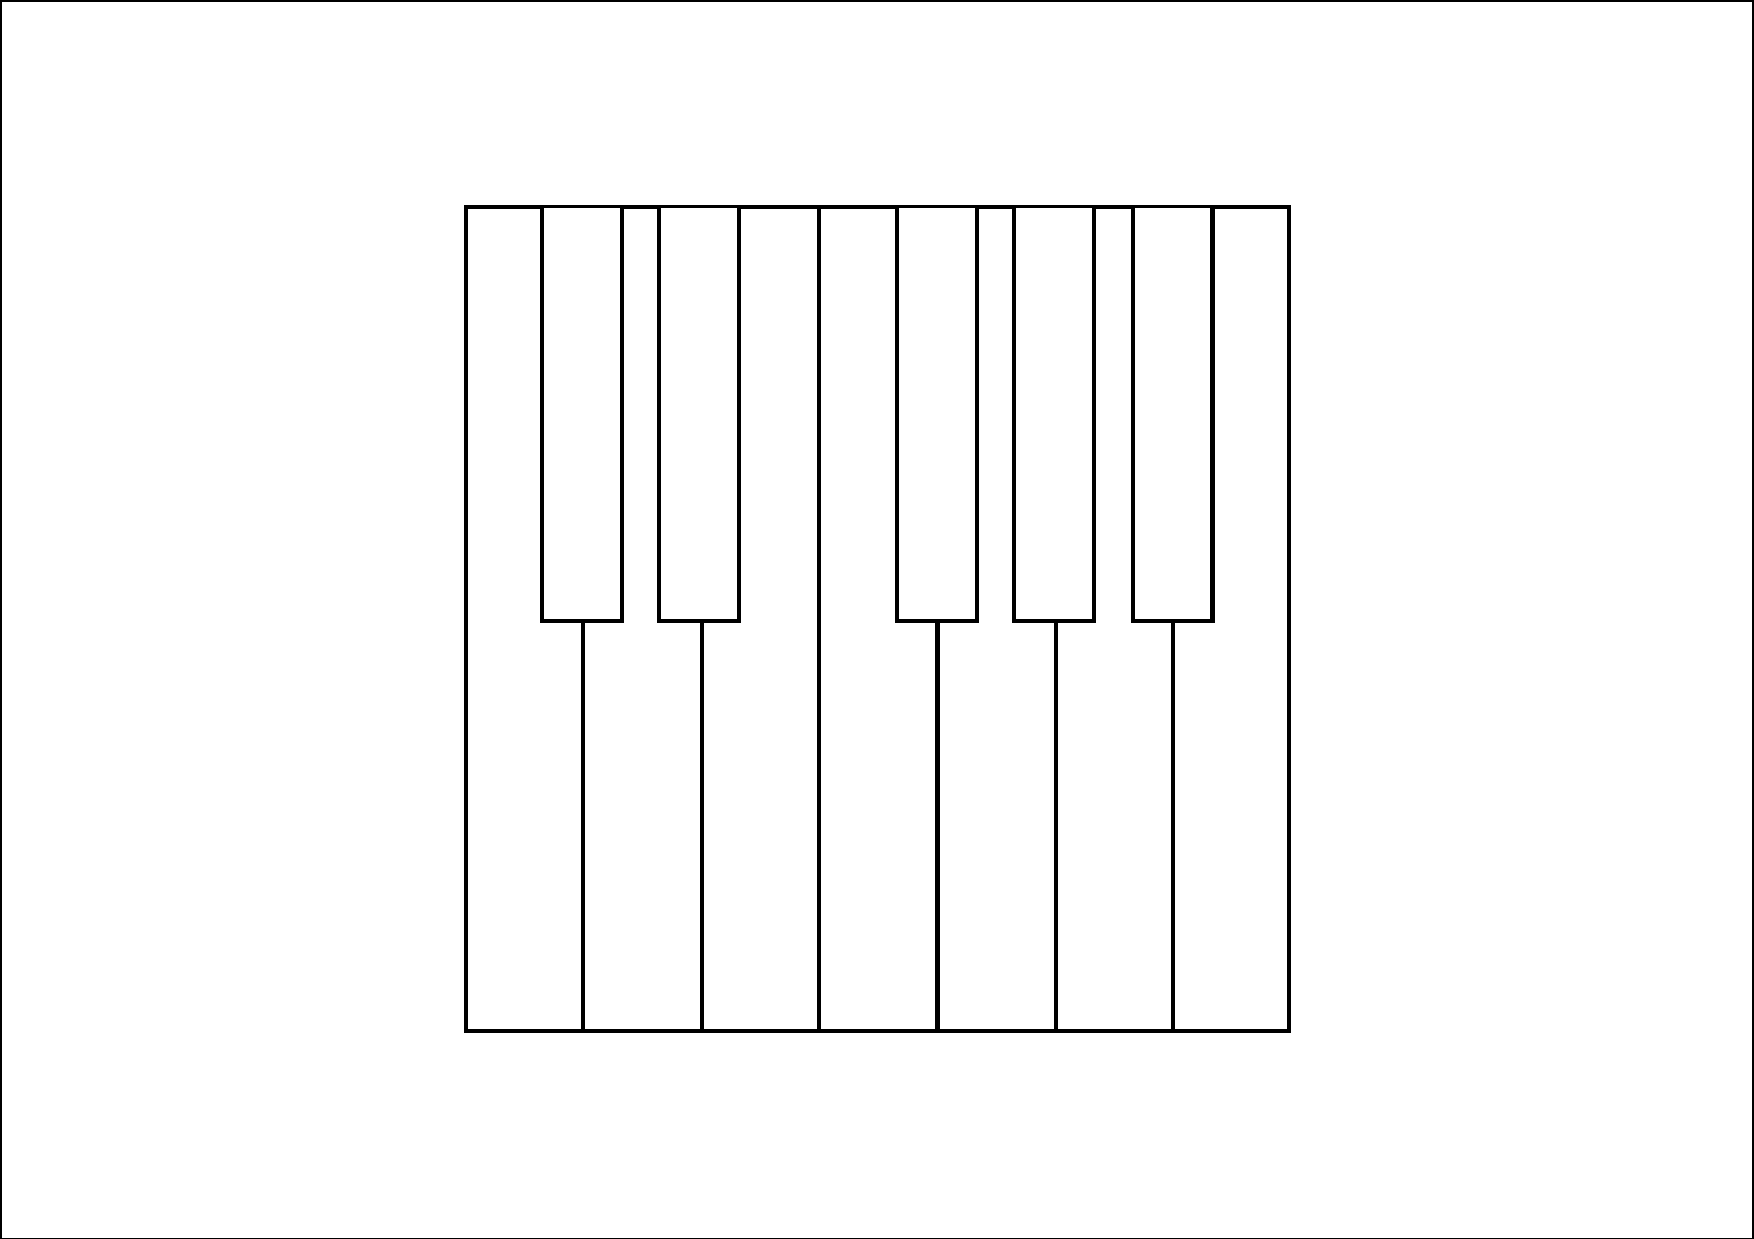
\includegraphics[width=\textwidth]{application/presets/keyboard-preset-1}
		\caption{}
		\label{fig:preset-1}
	\end{subfigure}
	\hfill
	\begin{subfigure}{0.49\textwidth}
		\centering
		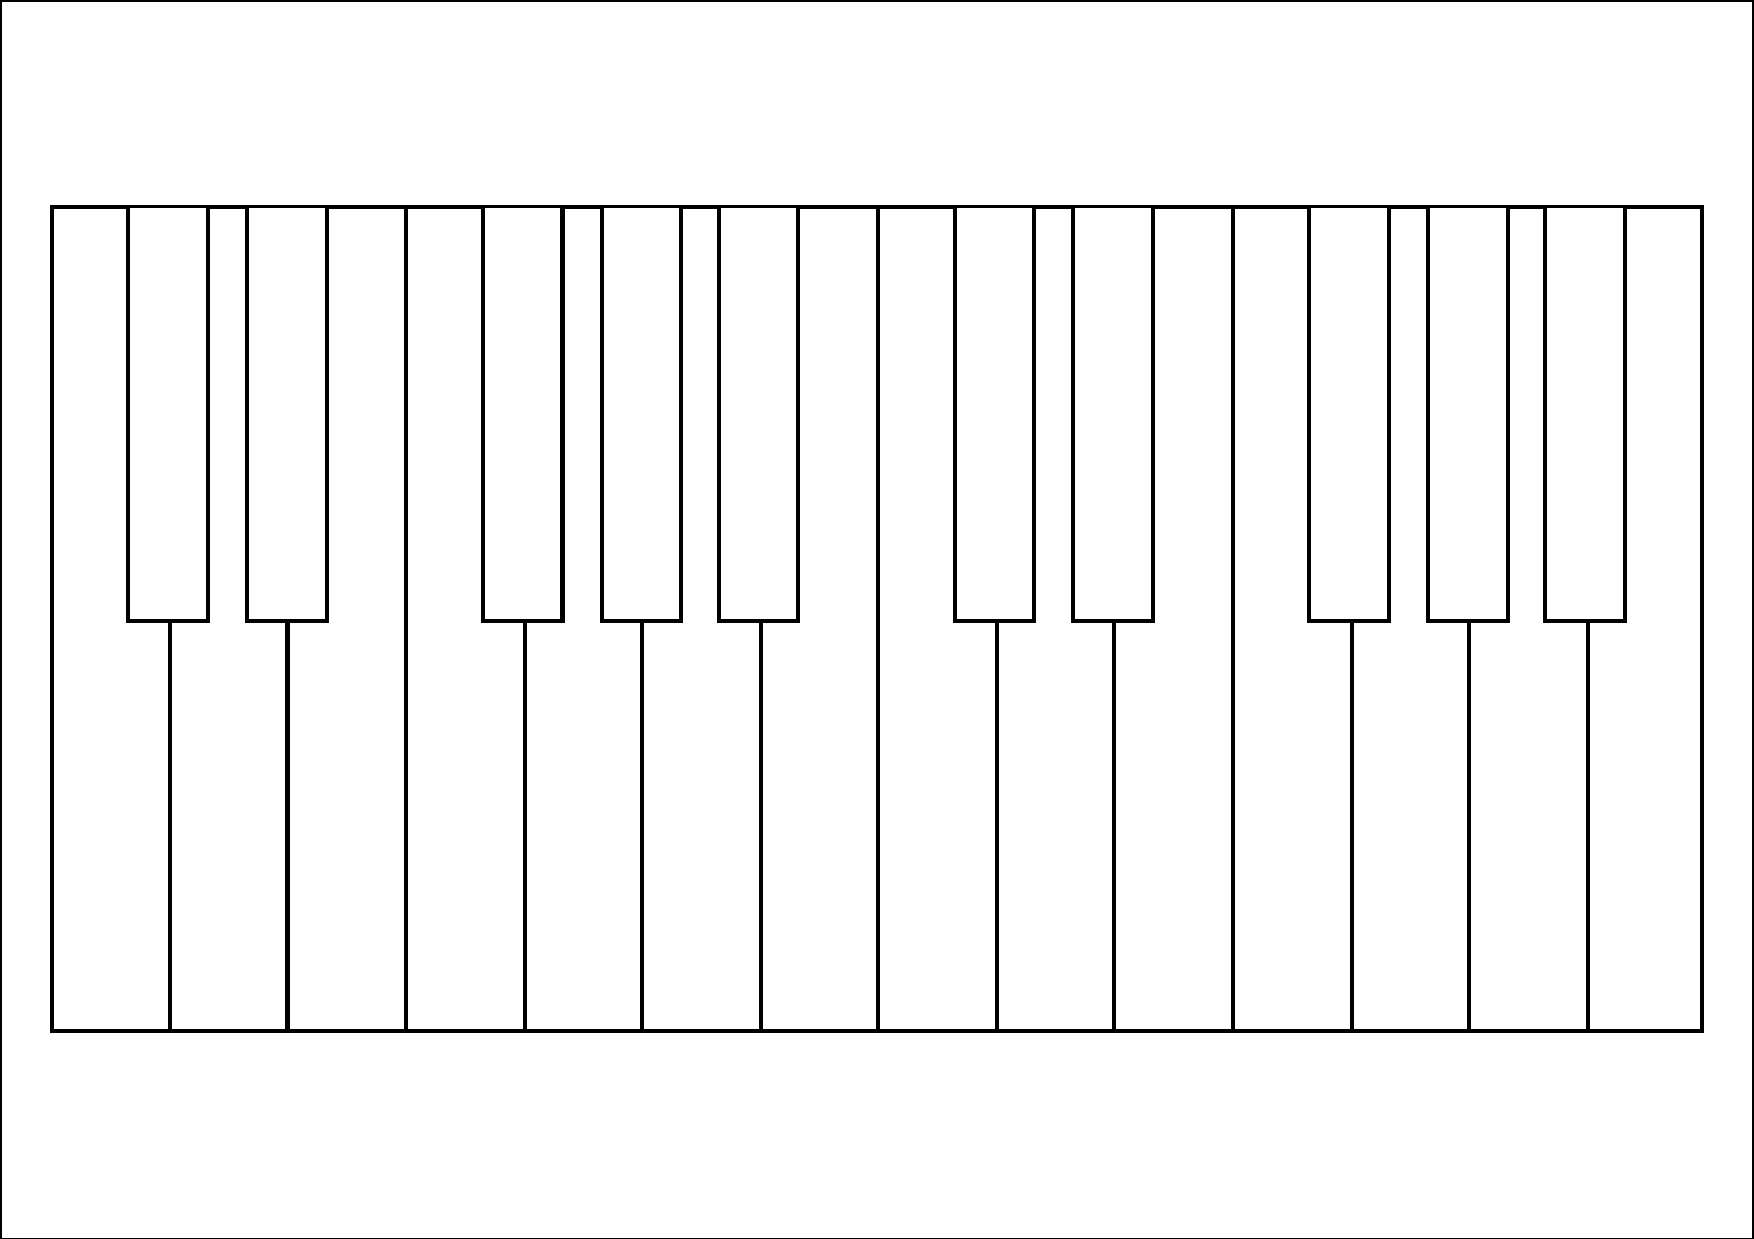
\includegraphics[width=\textwidth]{application/presets/keyboard-preset-2}
		\caption{}
		\label{fig:preset-2}
	\end{subfigure}
	\caption{
		Keyboard presets different keyboard sizes.
		(a) One octave keyboard;
		(b) Two octaves keyboard.
	}
	\label{fig:presets}
\end{figure}


\subsection{Real-time phase}\label{subsec:real-time-phase}
When the user is satisfied with the result of the detection phase, they can press a button to start the real-time phase.
First, the graph is launched: the GPU manager is started, models for palm detection,
hand landmarks and handedness are loaded, and side packets are created.
Three data streams are started from the graph: \textit{hand landmarks}, \textit{world hand landmarks} and
\textit{handedness}, and an event listener is attached to each to receive the results of the processing of each frame.
The graph is schematised in \autoref{fig:mediapipe-graph}.

\begin{figure}[ht]
	\centering
	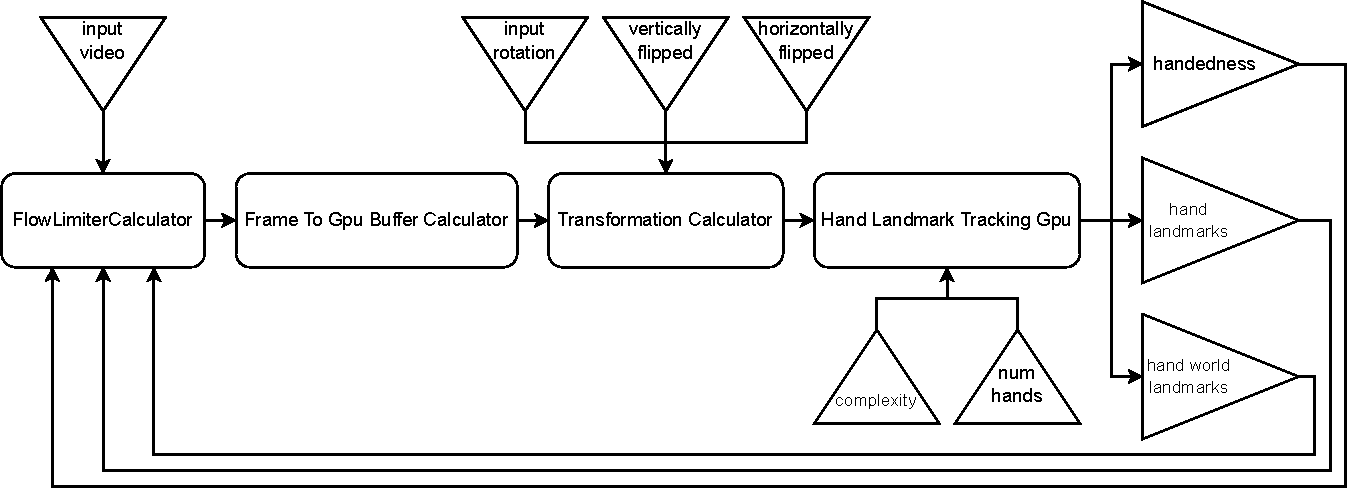
\includegraphics[width=\textwidth]{images/application/mediapipe-gpu}
	\caption{MediaPipe graph used in the application.}
	\label{fig:mediapipe-graph}
\end{figure}

The three data streams on which the outputs of the graph are passed work asynchronously
with respect to the main loop and also with respect to each other.
To ensure that the next step of the algorithm only starts when all three streams have produced a result
for the same frame, it was sufficient to implement a simple synchronisation system for the three outputs
to ensure that each frame is only passed to the next step of the algorithm when all three components are available.

Once all three components are available, our algorithm proceeds in its two phases:
\begin{itemize}
	\item \textit{Touch detection:} check if a finger touched the keyboard
	\item \textit{Note detection:} if a finger touched the keyboard,
	find which note was pressed and play the corresponding sound
\end{itemize}

It is important to note that, in its current state, not all three streams are used by our algorithm.
In particular, only the ones for \textit{hand landmarks} and \textit{handedness} are useful for our purposes.
The other, \textit{world hand landmarks}, is present mainly for reasons of compatibility with older
versions of the algorithm and the possibility that it will be useful in the future.

\paragraph{MediaPipe on low-end devices}
While the webcam and the video feed on the smartphone interface work at 30 FPS,
the frequency at which frames are sent to MediaPipe for hand detection is not fixed.
In order to meet all requirements and to be able to support as many smartphones as possible,
even low-end ones, we have implemented a way for the user to set the frequency at which frames are sent to
MediaPipe at will, i.e.\ the FPS at which the hand detection process runs.

This has been done by including buttons in the interface to directly increase and decrease the FPS with which to run MediaPipe.
Changing the value from the interface results in an immediate change in the operation of MediaPipe.

Through experimentation, we have found that a good value for MediaPipe's FPS is 15, which is high enough
to ensure that the app runs smoothly with low response times, but is not too high to be unusable on mid-range smartphones.

Going below 15 FPS is possible, but results in an increase in the app's response time and a possible loss of some notes.
Going above 15 FPS is also possible, and it is recommended in the case of high-end smartphones,
but being aware that increasing the frequency with which frames are sent to
MediaPipe also increases battery consumption and could lead to the smartphone overheating.

\subsubsection{Touch detection}
At this early stage of the project, the touch detection procedure is not yet very refined.
Since MediaPipe alone does not provide sufficiently precise depth coordinates (or camera distance) but rather
inconsistent and flickering ones, and for the reasons explained in \autoref{subsec:mp-for-3d}~\nameref{subsec:mp-for-3d},
we could not rely solely on them for the touch detection phase.
We therefore exploit the advantages explained in \autoref{subsec:pov}~\nameref{subsec:pov}.

To detect a touch, we rely on the position of the finger on the $y_s$ axis: when a finger reaches
down towards the paper to play a note, this movement is detected by MediaPipe thanks to the 45\degree \ view.
The $y_s$ position of the finger is given as input to an automaton that takes care
of maintaining and updating the state of the finger at each frame.
The automaton is illustrated in \autoref{fig:touch-automata}.

When a new frame is ready, the $x_s$ and $y_s$ positions of the finger are extracted from MediaPipe
and converted into pixels and the $y_s$ position is given to the automaton.
The automaton calculates the speed of the finger by comparing the new $y_s$ with the last detected $y_s$,
after which it advances the finger state accordingly.
When the finger enters the \textit{Touching} state, the $x_s$ and $y_s$ coordinates are passed to the note detector
which is responsible for verifying that the finger has touched a key and, if so, playing the corresponding note.
The automaton is made so that the \textit{Touching} state remains active even if the finger moves horizontally.

In \autoref{fig:touch-automata}, the \texttt{t} value indicates a threshold which serves to mitigate the instability of MediaPipe:
the hand landmarks detected by MediaPipe are subject to minute, continuous variations which, if not taken into account,
would cause a series of false positives and would repeatedly take the automaton in and out of the \textit{Touching} state.
Experimentally, we came to the conclusion that 8 is a suitable value for the automaton's activation threshold.

The pseudocode for this phase is shown in~\autoref{alg:touch-detection}.

\begin{algorithm}
	\caption{Touch detection}
	\begin{algorithmic}[1]
		\State when new frame arrives
		\If{no hand has been detected}
			\State \Return
		\EndIf
		\State $toPlay \gets \{\}$
		\For{each hand $h$ detected}
			\For{each finger $f$ of $h$}
				\State $x \gets$ horizontal position of $f$
				\State $y \gets$ vertical position of $f$
				\State $isPlaying \gets$ automata($f$).update($y$)
				\If{$isPlaying$}
					\State $toPlay \gets toPlay \ \bigcup \ \left\{ \left( x, y \right) \right\}$
				\EndIf
			\EndFor
		\EndFor
		\State do \textit{note detection} with $toPlay$
	\end{algorithmic}
	\label{alg:touch-detection}
\end{algorithm}

\begin{figure}[ht]
	\centering
	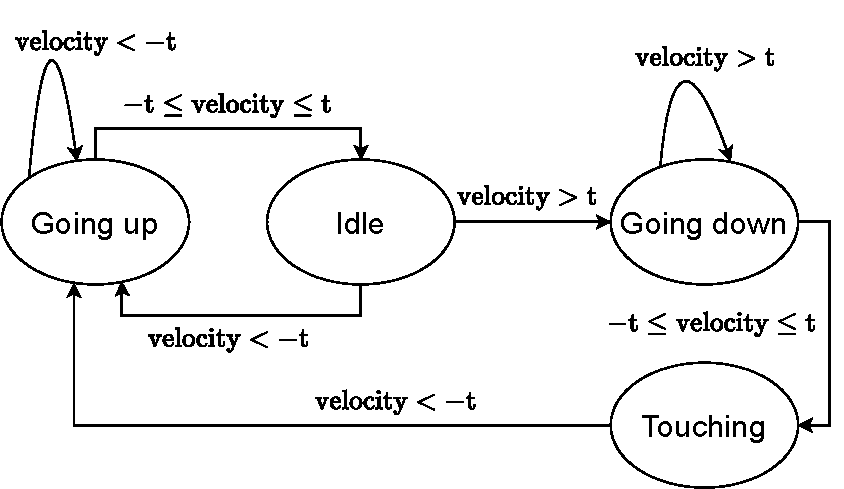
\includegraphics[width=\textwidth]{images/application/touch-automata}
	\caption{The automata used to detect finger touch.}
	\label{fig:touch-automata}
\end{figure}

\subsubsection{Note detection}\label{subsubsec:notes-detection}
Once we have detected the fingers touching the keyboard with MediaPipe,
we need to work out which notes have been touched.
To do this, we use the image generated in the keyboard detection phase in
\autoref{par:notes-detection}~\nameref{par:notes-detection}.

This image is the same size as the video feed and is totally black except where the keys are located.
The keys are coloured in a grey scale where the first key is coloured with the value 1,
the second with the value 2 and so on.
This allows us to associate each key with a unique value that we can use to determine the note to be played.

Using the $x_s$ and $y_s$ coordinates provided by MediaPipe, we can superimpose them on the image generated
in the keyboard detection phase to determine whether a finger has touched a key.
If the pixel at position $(x, y)$ is black, the finger is outside the keyboard and nothing happens.
If, on the other hand, the pixel is not black, the finger is on one of the detected keys and therefore the MIDI signal
corresponding to the detected note at that position must be played.

Playing sounds is not as straightforward a process as it might seem, and it does require a little forethought.
This is because when passing from one frame to another, some fingers that were playing
in the previous frame may still be playing the same key.
In this case the note does not have to be played again, but only continued.

To do this, we keep a list of the notes that are being played and, at each frame, create two different sets of notes:
the set of notes that were being played in the previous frame but are no longer being played in the current frame,
and the set of notes that were not being played in the previous frame but are being played in the current frame.

This allows to detect notes that were being played in the previous frame and are still being played in the current frame,
so that they are not played again but remain playing.

The pseudocode for this phase is shown in~\autoref{alg:note-detection}.

\begin{algorithm}
	\caption{Note detection}
	\begin{algorithmic}[1]
		\State \textbf{Input}: the set of coordinates $toPlay$ of the fingers touching the keyboard
		\State $playing \gets \{n \ | \ n \text{ is already being played from the previous frame}\}$
		\State $detected \gets \{ n \ | \ (x, y) \in toPlay \text{ and }\newline
		\hspace*{21.6mm} n \text{ is a non-black pixel at } (x, y) \text{ in the note image}\}$
		\State $stop \gets playing \setminus detected$
		\State $start \gets detected \setminus playing$
		\For{each $n$ in $stop$}
			\State stop playing note $n$
		\EndFor
		\For{each $n$ in $start$}
			\State start playing note $n$
		\EndFor
	\end{algorithmic}
	\label{alg:note-detection}
\end{algorithm}

\begin{figure}[ht]
	\centering
	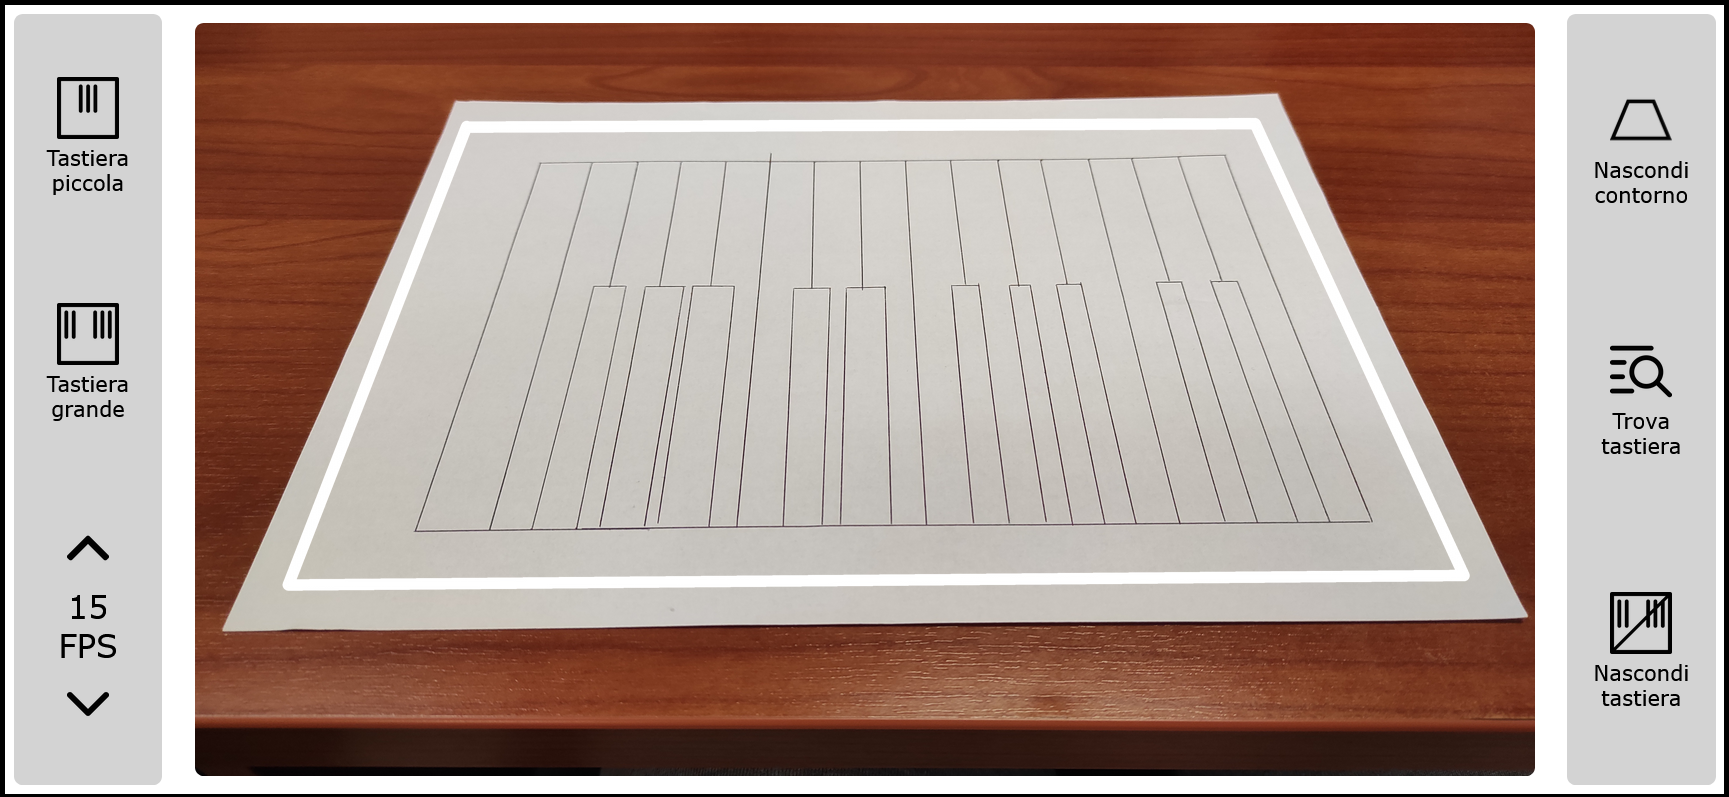
\includegraphics[width=\textwidth]{images/application/screenshots/detection-phase}
	\caption{Application during detection phase, with perimeter visible.}
	\label{fig:screenshot-detection-phase}
\end{figure}

\begin{figure}[ht]
	\centering
	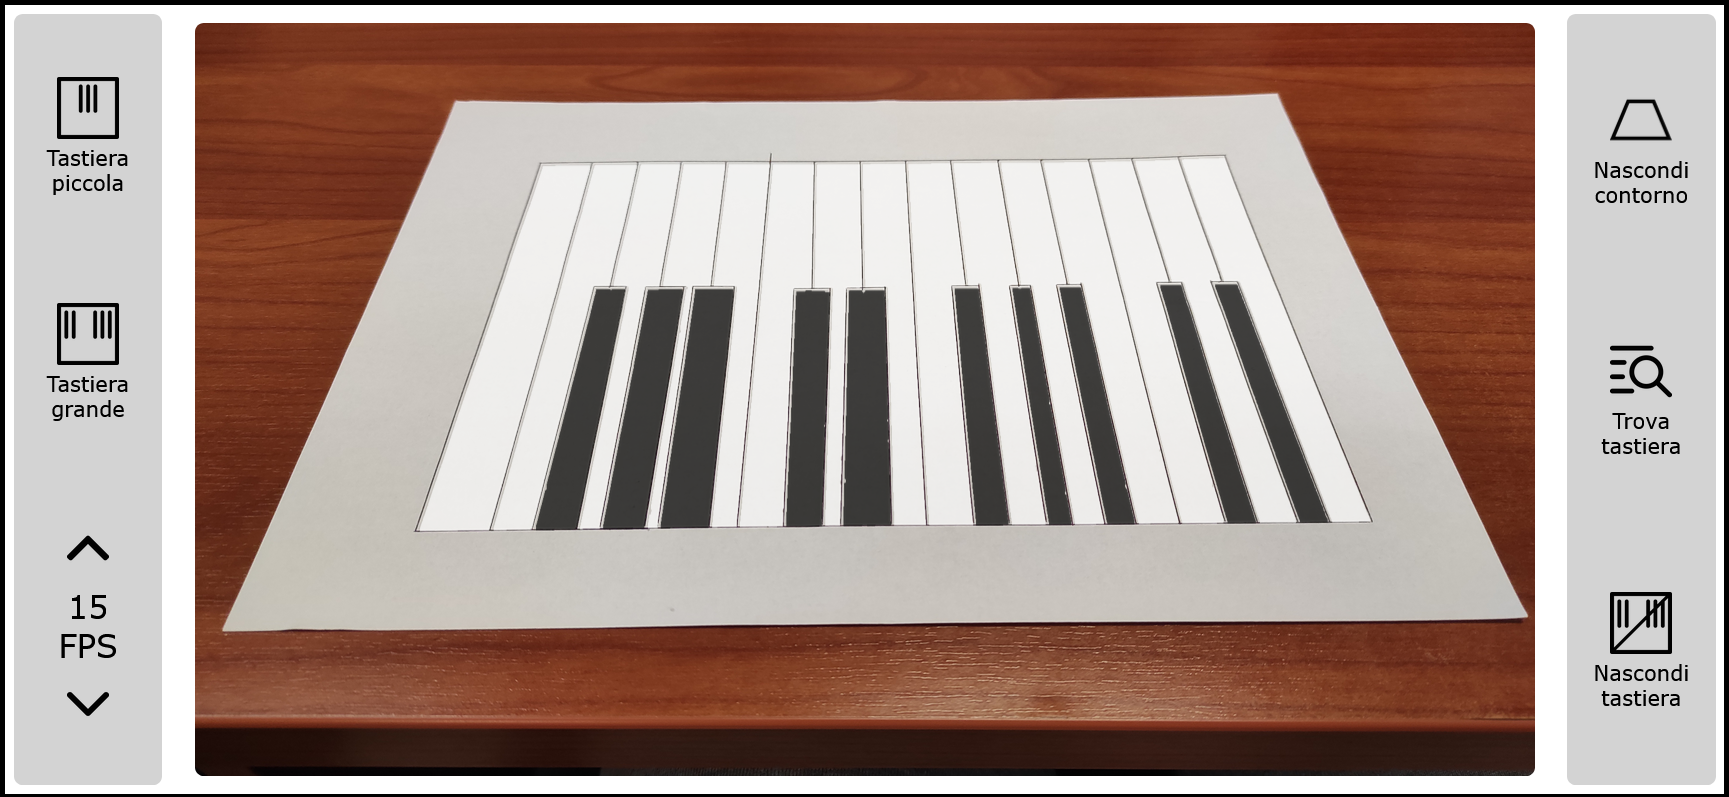
\includegraphics[width=\textwidth]{images/application/screenshots/playing-phase}
	\caption{Application after keyboard detection, with keyboard overlay visible.}
	\label{fig:screenshot-playing-phase}
\end{figure}

